% Options for packages loaded elsewhere
\PassOptionsToPackage{unicode}{hyperref}
\PassOptionsToPackage{hyphens}{url}
\PassOptionsToPackage{dvipsnames,svgnames,x11names}{xcolor}
%
\documentclass[
  13pt,
  ignorenonframetext,
]{beamer}
\usepackage{pgfpages}
\setbeamertemplate{caption}[numbered]
\setbeamertemplate{caption label separator}{: }
\setbeamercolor{caption name}{fg=normal text.fg}
\beamertemplatenavigationsymbolsempty
% Prevent slide breaks in the middle of a paragraph
\widowpenalties 1 10000
\raggedbottom
\setbeamertemplate{part page}{
  \centering
  \begin{beamercolorbox}[sep=16pt,center]{part title}
    \usebeamerfont{part title}\insertpart\par
  \end{beamercolorbox}
}
\setbeamertemplate{section page}{
  \centering
  \begin{beamercolorbox}[sep=12pt,center]{part title}
    \usebeamerfont{section title}\insertsection\par
  \end{beamercolorbox}
}
\setbeamertemplate{subsection page}{
  \centering
  \begin{beamercolorbox}[sep=8pt,center]{part title}
    \usebeamerfont{subsection title}\insertsubsection\par
  \end{beamercolorbox}
}
\AtBeginPart{
  \frame{\partpage}
}
\AtBeginSection{
  \ifbibliography
  \else
    \frame{\sectionpage}
  \fi
}
\AtBeginSubsection{
  \frame{\subsectionpage}
}
\usepackage{amsmath,amssymb}
\usepackage{lmodern}
\usepackage{iftex}
\ifPDFTeX
  \usepackage[T1]{fontenc}
  \usepackage[utf8]{inputenc}
  \usepackage{textcomp} % provide euro and other symbols
\else % if luatex or xetex
  \usepackage{unicode-math}
  \defaultfontfeatures{Scale=MatchLowercase}
  \defaultfontfeatures[\rmfamily]{Ligatures=TeX,Scale=1}
\fi
% Use upquote if available, for straight quotes in verbatim environments
\IfFileExists{upquote.sty}{\usepackage{upquote}}{}
\IfFileExists{microtype.sty}{% use microtype if available
  \usepackage[]{microtype}
  \UseMicrotypeSet[protrusion]{basicmath} % disable protrusion for tt fonts
}{}
\makeatletter
\@ifundefined{KOMAClassName}{% if non-KOMA class
  \IfFileExists{parskip.sty}{%
    \usepackage{parskip}
  }{% else
    \setlength{\parindent}{0pt}
    \setlength{\parskip}{6pt plus 2pt minus 1pt}}
}{% if KOMA class
  \KOMAoptions{parskip=half}}
\makeatother
\usepackage{xcolor}
\newif\ifbibliography
\usepackage{graphicx}
\makeatletter
\def\maxwidth{\ifdim\Gin@nat@width>\linewidth\linewidth\else\Gin@nat@width\fi}
\def\maxheight{\ifdim\Gin@nat@height>\textheight\textheight\else\Gin@nat@height\fi}
\makeatother
% Scale images if necessary, so that they will not overflow the page
% margins by default, and it is still possible to overwrite the defaults
% using explicit options in \includegraphics[width, height, ...]{}
\setkeys{Gin}{width=\maxwidth,height=\maxheight,keepaspectratio}
% Set default figure placement to htbp
\makeatletter
\def\fps@figure{htbp}
\makeatother
\setlength{\emergencystretch}{3em} % prevent overfull lines
\providecommand{\tightlist}{%
  \setlength{\itemsep}{0pt}\setlength{\parskip}{0pt}}
\setcounter{secnumdepth}{-\maxdimen} % remove section numbering
%\ProvidesPackage{config/presento}

\mode<presentation>

% removing navigation symbols
\setbeamertemplate{navigation symbols}{}

% packages
\usepackage{xcolor}
\usepackage{fontspec}
\usepackage{setspace}
\usepackage{tikz}
\usepackage{multicol}
\usepackage{multirow}
\usepackage{philex}

% colors
\definecolor{colorblack}{HTML}{000000} % for note
\definecolor{colorgreen}{HTML}{009933} % for code
\definecolor{colorwhite}{HTML}{FFFFFF} % background
\definecolor{colorblue}{HTML}{0099CC} % blue
\definecolor{colorbig}{HTML}{1f77b4} % for note
\definecolor{colormedium}{HTML}{ff7f0e} % for note
\definecolor{colorsmall}{HTML}{2ca02c} % for note


% font sizes
\newcommand{\fontsizeone}{1em}
\newcommand{\fontsizetwo}{0.85em}
\newcommand{\fontsizethree}{1em}
% line spaces
\newcommand{\linespaceone}{1}

% font families
\newfontfamily{\inconsolatafont}[Path=fonts/]{brill}

% beamer template changes
\setbeamertemplate{frametitle}{
 \vspace{0.40em}
 \noindent
 \hspace{-1.22em}
 \tikz[overlay,remember picture,baseline=0.3em]{\fill[fill= colorblue]  (-0.3,0.05) rectangle (0,0.9); }\color{colorblue}~~\insertframetitle%
}

\setmainfont[Ligatures=TeX,Path=fonts/,
						BoldFont=brillb,
						ItalicFont=brilli,
						BoldItalicFont=brillbi,
						SmallCapsFont=brill]{brill}
\setsansfont[Ligatures=TeX,Path=fonts/,
						BoldFont=brillb,
						ItalicFont=brilli,
						BoldItalicFont=brillbi,
						SmallCapsFont=brill]{brill}
\setmonofont[Scale=0.7, Path=fonts/]{iosevka-regular}

% frame counter
\newcounter{totalfr}
\setbeamertemplate{footline}{
  \ifnum\inserttotalframenumber=1
    \setcounter{totalfr}{2}
  \else
     \setcounter{totalfr}{\inserttotalframenumber}
  \fi
  \hfill{
    \tikz{
      \filldraw[fill=colorblue!80, draw=colorblue!80]  (0,0) -- (0.2,0) arc (0:{\value{framenumber}*(360/(\value{totalfr}))}:0.2) -- (0,0); 
      \node at (0,0) {\normalsize \color{colorblack}\tiny{\insertframenumber}};
    }
  }
  \hspace{2em}
  \vspace*{1em}
}

% custom commands
\newcommand{\hugetext}[1]{
  {
  \begin{spacing}{\linespaceone}
   \fontsize{\fontsizeone}{\fontsizeone}{ #1}
  \end{spacing}
  }
}

\newcommand{\largetext}[1]{
 {\fontsize{\fontsizetwo}{\fontsizeone}\selectfont{#1}}
}

\newcommand{\setnote}[1]{
 {\fontsize{\fontsizethree}{\fontsizeone}\selectfont\color{colorblack}{#1}}
}

\newcommand{\framecard}[2][colorblue]{
  {\setbeamercolor{background canvas}{bg=#1}
    \begin{frame}[plain]
    \vfill
    \begin{center}
     {#2}
    \end{center}
    \vfill
    \end{frame}
  }
}
\newcommand{\framepic}[3][1]{
  {
    \usebackgroundtemplate{%
    \tikz[overlay,remember picture] \node[opacity=#1, at=(current page.center)] {
      \includegraphics[width=\paperwidth]{#2}};
    }
    \begin{frame}
    #3
    \end{frame}
  }
}

\setbeamercolor{background canvas}{bg=colorwhite}
\setbeamercolor{normal text}{fg=colorblack}
\setbeamercolor{title}{fg=colorblue}
\setbeamercolor{subtitle}{fg=colorblue}
\setbeamercolor{author}{fg=colorblack}
\setbeamercolor{alerted text}{fg=colorblue}

\defbeamertemplate*{title page}{customized}[1][]
{
  \vfill
  {\usebeamercolor[fg]{title}\hugetext{\inserttitle}}
  {\usebeamerfont{subtitle}\usebeamercolor[fg]{subtitle}\largetext{\insertsubtitle}\par}
  \vfill
  {\usebeamercolor[fg]{author}\largetext{\insertauthor}}\\
  {\setnote{\insertinstitute}\par}
  \vfill
  {\setnote{\insertdate}\par}
  \vfill
}

\usepackage{natbib}
\bibpunct[: ]{(}{)}{;}{a}{}{,}

\setbeamertemplate{itemize items}{\color{colorblue}$\bullet$}
\setbeamertemplate{enumerate items}{\color{colorblue}$\theenumi$.}
\setbeamertemplate{frametitle continuation}{}
\setbeamercolor{block title}{fg=colorblue,bg=white} 

\usepackage{hyperref}
\hypersetup{linkcolor=colorblue, colorlinks=true}

\AtBeginSection[]
{
  \begin{frame}
    \frametitle{Outline of the talk}
    \tableofcontents[currentsection]
  \end{frame}
}

\setbeamertemplate{caption}{\raggedright\insertcaption\par}
\ifLuaTeX
  \usepackage{selnolig}  % disable illegal ligatures
\fi
\usepackage[]{natbib}
\bibliographystyle{plainnat}
\IfFileExists{bookmark.sty}{\usepackage{bookmark}}{\usepackage{hyperref}}
\IfFileExists{xurl.sty}{\usepackage{xurl}}{} % add URL line breaks if available
\urlstyle{same} % disable monospaced font for URLs
\hypersetup{
  pdftitle={Международная лаборатория языковой конвергенции},
  pdfauthor={Г. А. Мороз},
  colorlinks=true,
  linkcolor={Maroon},
  filecolor={Maroon},
  citecolor={colorblue},
  urlcolor={colorblue},
  pdfcreator={LaTeX via pandoc}}

\title{Международная лаборатория языковой конвергенции}
\author{Г. А. Мороз}
\date{24 ноября 2022}

\begin{document}
\frame{\titlepage}

\begin{frame}{О лаборатории}
\protect\hypertarget{ux43e-ux43bux430ux431ux43eux440ux430ux442ux43eux440ux438ux438}{}
\begin{itemize}
\tightlist
\item
  Открыта в 2017 году
\end{itemize}

\begin{figure}

{\centering 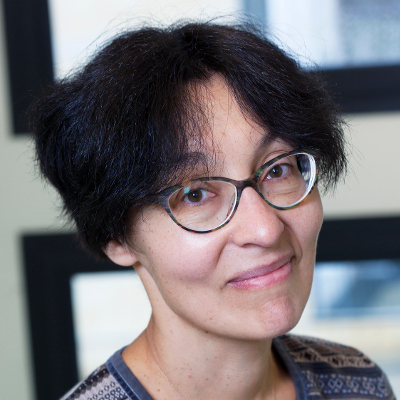
\includegraphics[width=0.4\linewidth]{images/01_dobrushina} 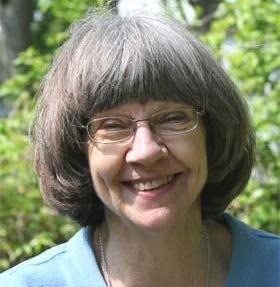
\includegraphics[width=0.4\linewidth]{images/02_nichols} 

}

\caption{Н. Р. Добрушина и Дж. Николс}\label{fig:unnamed-chunk-2}
\end{figure}

Оба исследователя специализируются на славянских языках и языках
Кавказа, а также лингвистической типологии

\begin{itemize}
\tightlist
\item
  C июля 2022 новый заведующий
\end{itemize}
\end{frame}

\begin{frame}{Миссия}
\protect\hypertarget{ux43cux438ux441ux441ux438ux44f}{}
Исследование механизмов конвергентных процессов в истории языка, то есть
языковых ситуаций, при которых контакт между носителями разных языков
ведет к появлению у этих языков общих черт. В лаборатории
разрабатываются инструменты для выявления результатов таких процессов по
данным электронных корпусов устной речи и создаются каталоги таких
явлений на материале малых языков России.
\end{frame}

\begin{frame}{Состав}
\protect\hypertarget{ux441ux43eux441ux442ux430ux432}{}
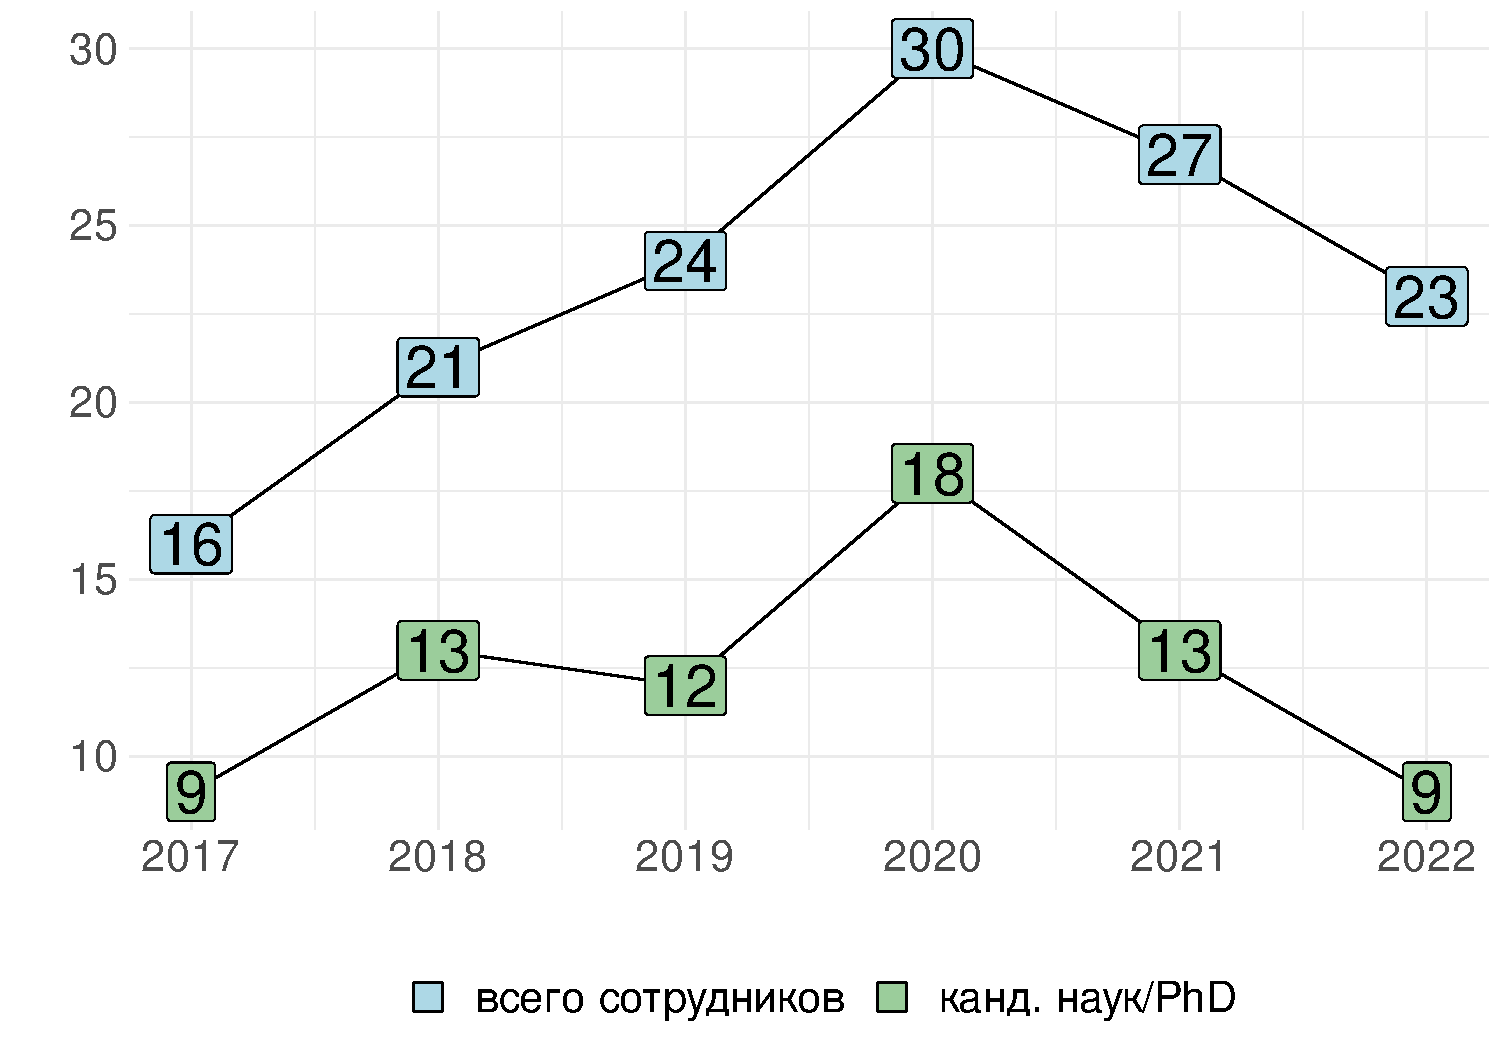
\includegraphics{2023.11.24_moroz_conlab_HSE_experts_files/figure-beamer/unnamed-chunk-3-1.pdf}
\end{frame}

\begin{frame}{Основные проекты}
\protect\hypertarget{ux43eux441ux43dux43eux432ux43dux44bux435-ux43fux440ux43eux435ux43aux442ux44b}{}
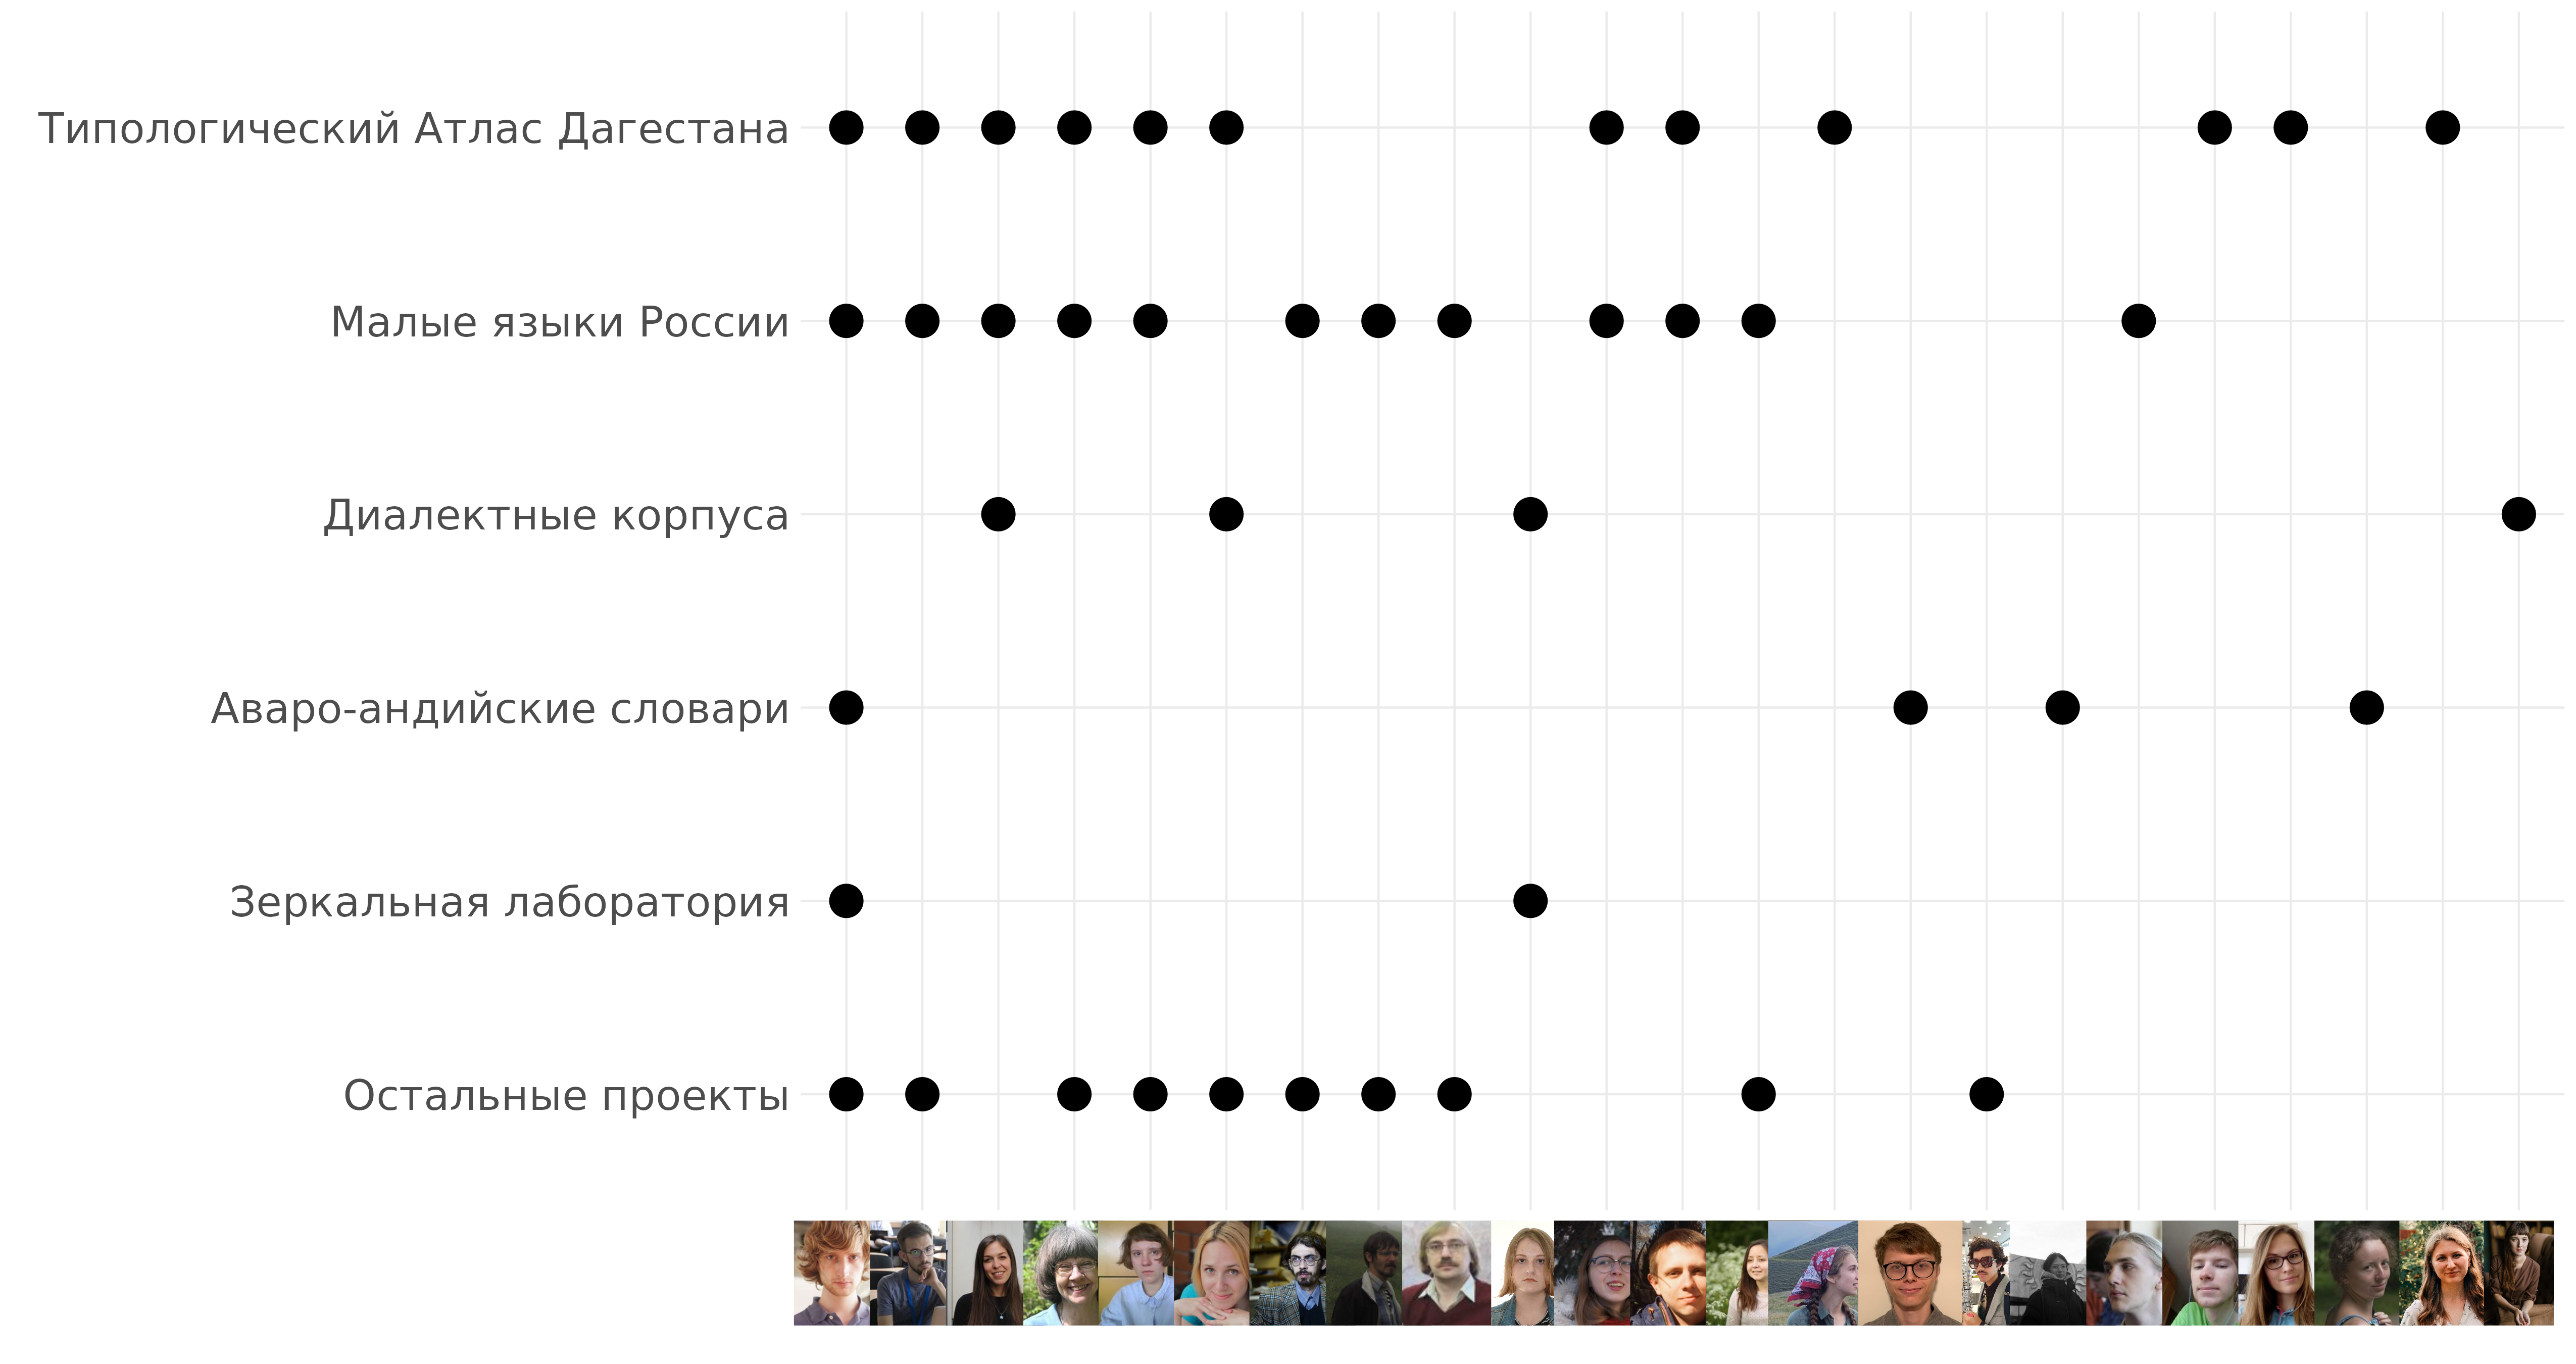
\includegraphics[width=1.1\linewidth]{images/03_projects}
\end{frame}

\begin{frame}{Типологический атлас Дагестана}
\protect\hypertarget{ux442ux438ux43fux43eux43bux43eux433ux438ux447ux435ux441ux43aux438ux439-ux430ux442ux43bux430ux441-ux434ux430ux433ux435ux441ux442ux430ux43dux430}{}
\begin{itemize}
\tightlist
\item
  48 глав, описывающих грамматические особенности языков Дагестана,
  каждая глава

  \begin{itemize}
  \tightlist
  \item
    прошла рецензирование
  \item
    содержит набор стандартизированных динамических карт
  \end{itemize}
\end{itemize}

\begin{center}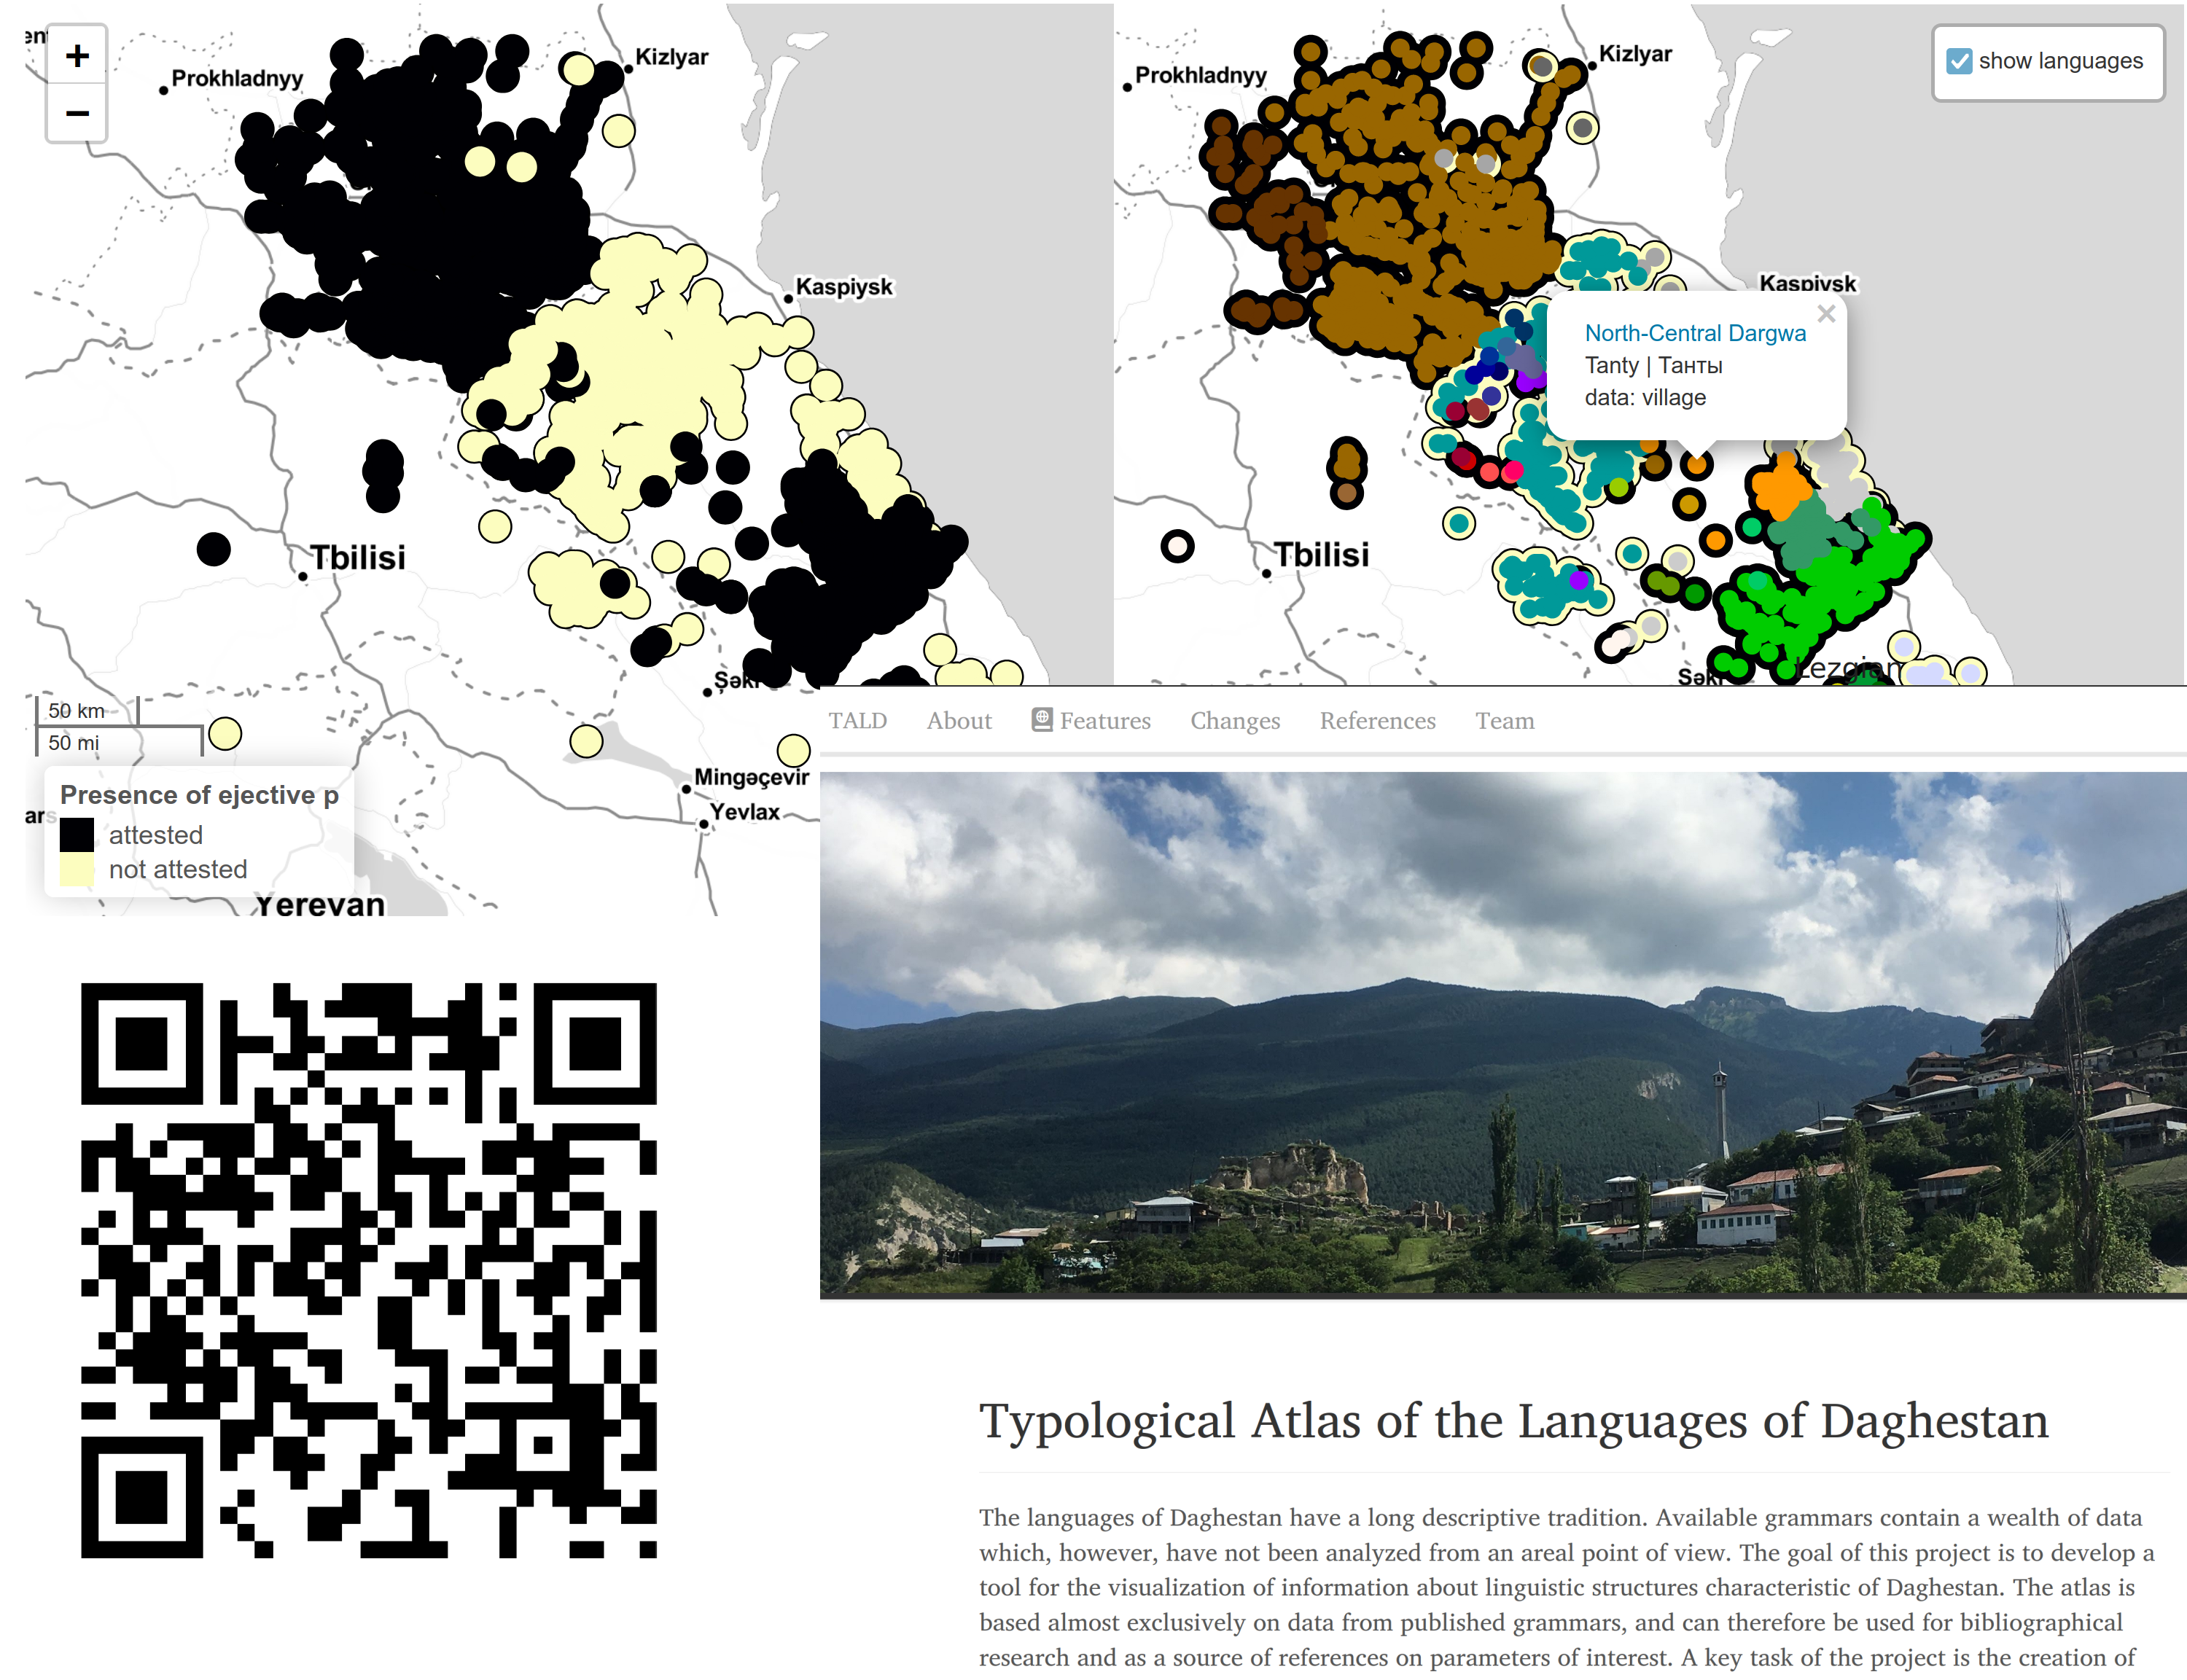
\includegraphics[width=0.8\linewidth]{images/04_tald} \end{center}
\end{frame}

\begin{frame}{Диалектные устные корпуса русского языка}
\protect\hypertarget{ux434ux438ux430ux43bux435ux43aux442ux43dux44bux435-ux443ux441ux442ux43dux44bux435-ux43aux43eux440ux43fux443ux441ux430-ux440ux443ux441ux441ux43aux43eux433ux43e-ux44fux437ux44bux43aux430}{}
\begin{itemize}
\tightlist
\item
  15 диалектных устных корпусов русского языка
\item
  7 устных корпусов билингвального русского
\end{itemize}

\begin{center}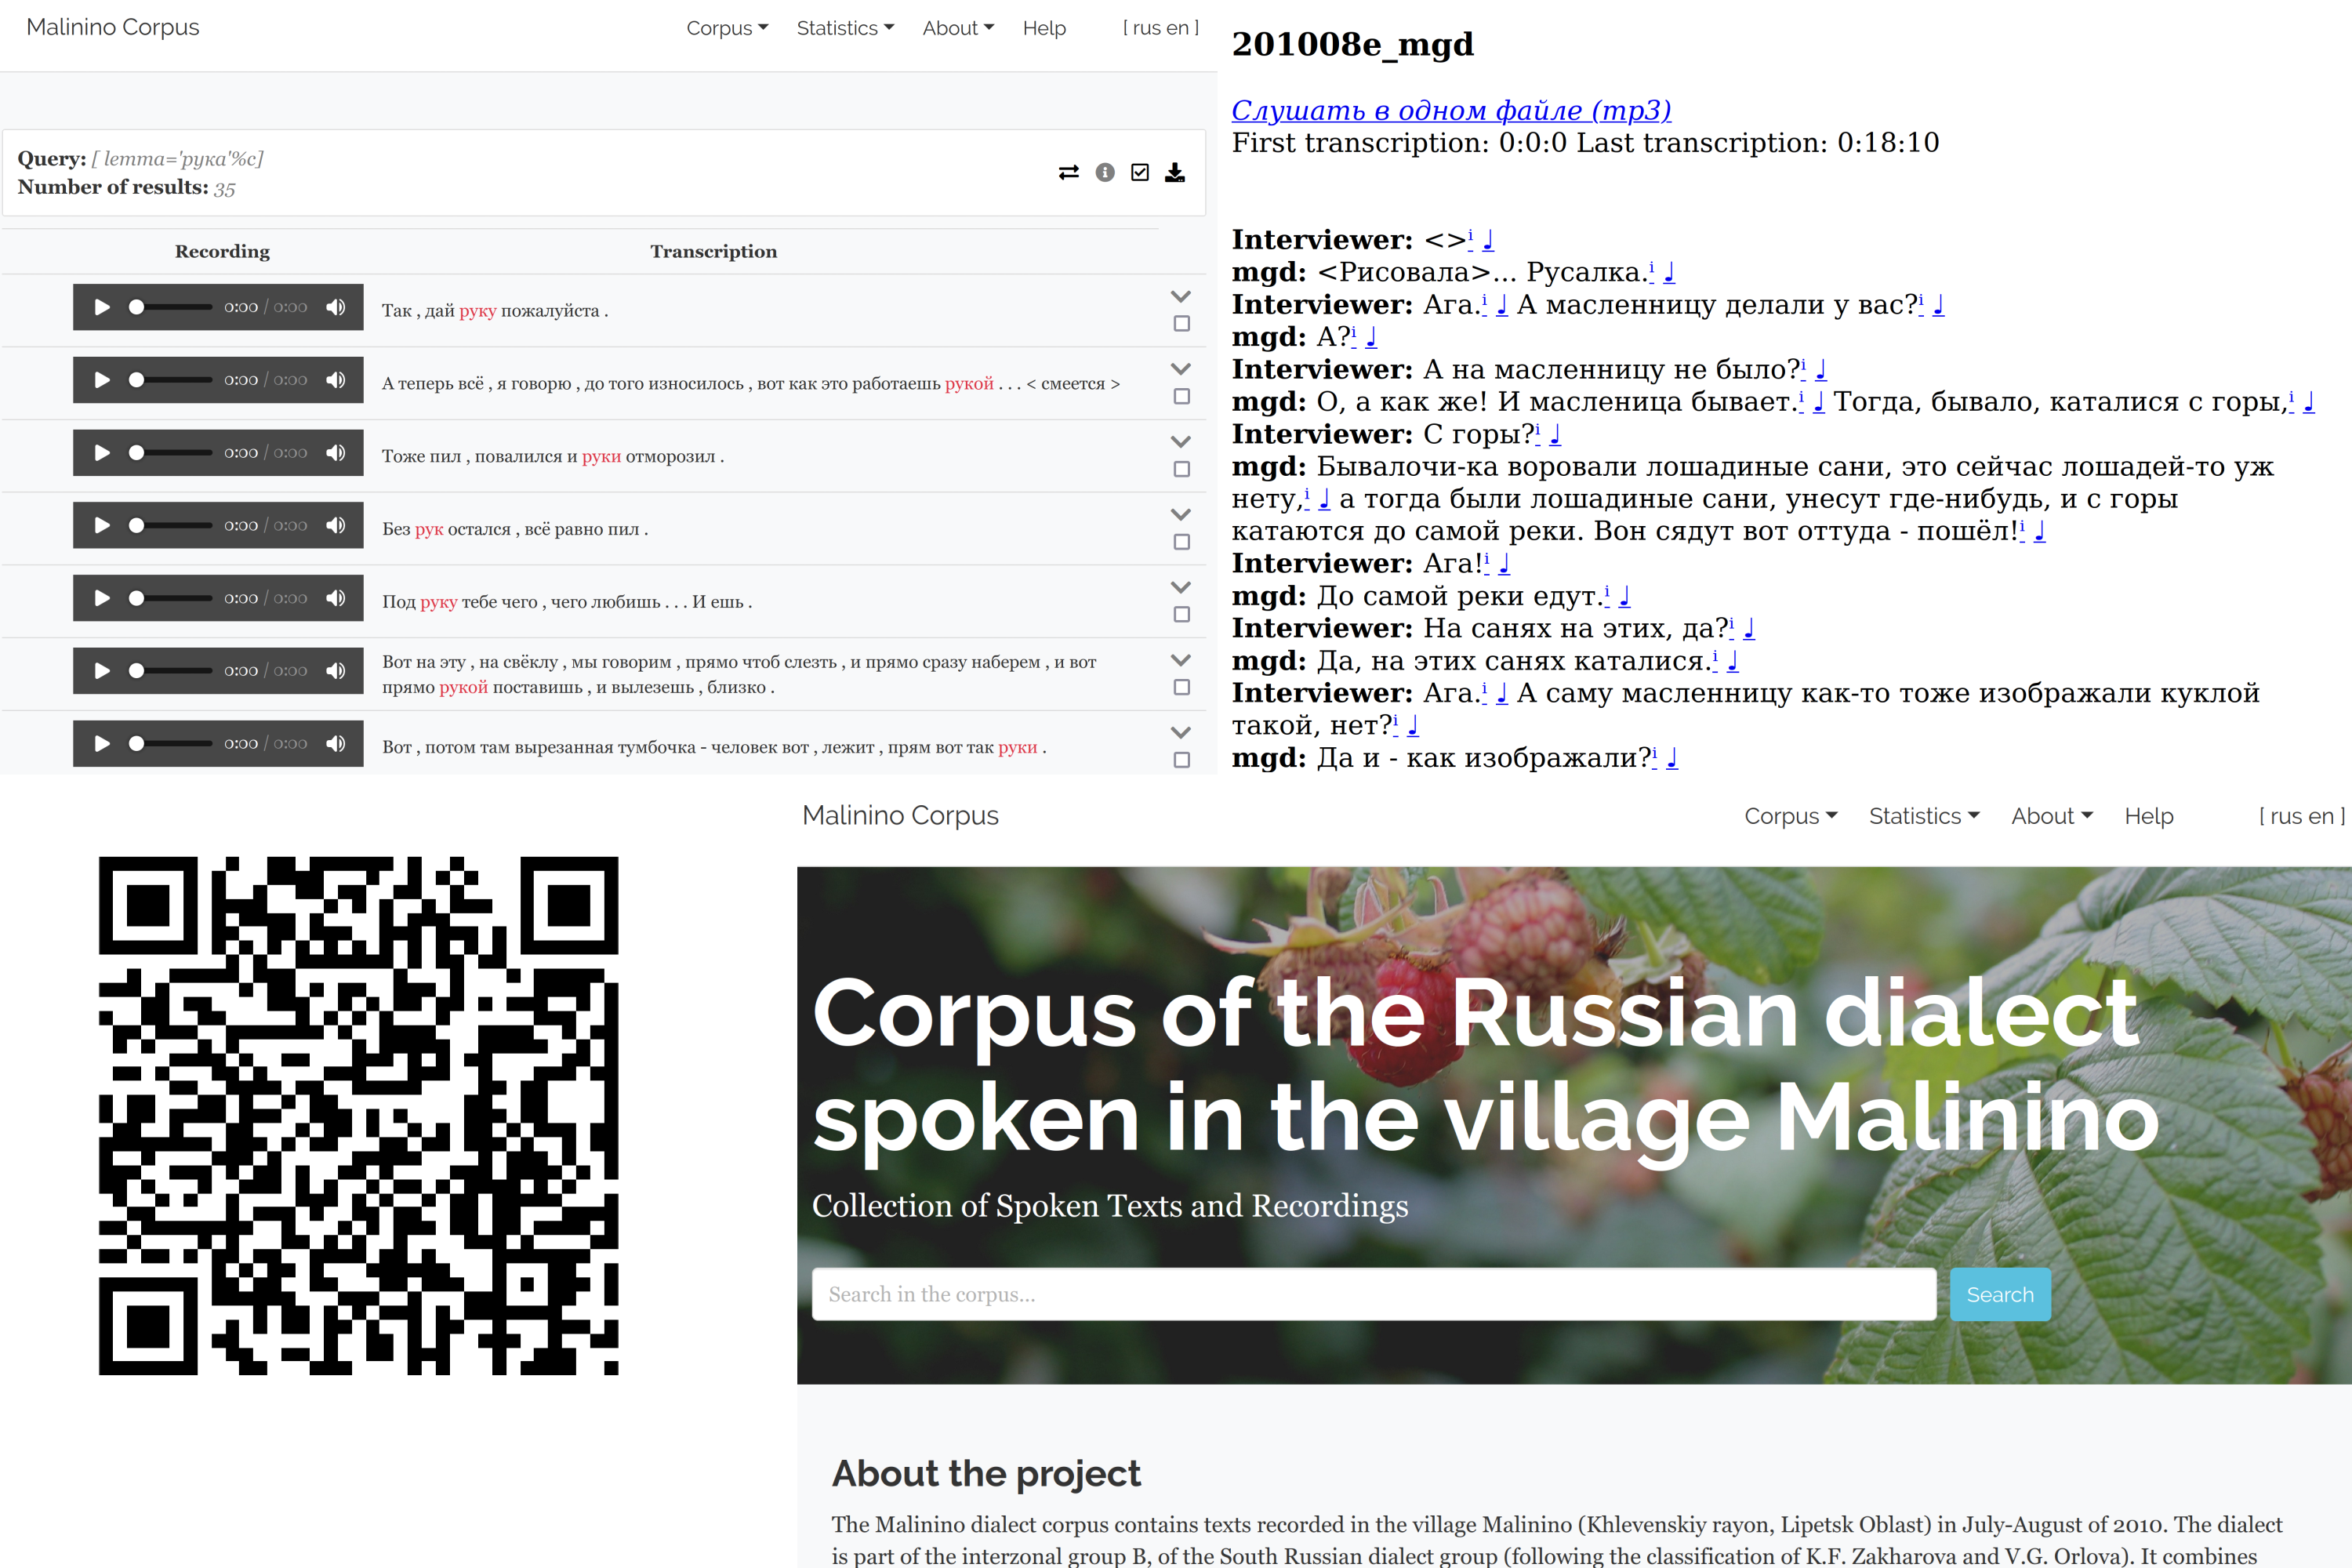
\includegraphics[width=1\linewidth]{images/05_corpus} \end{center}
\end{frame}

\begin{frame}{105 семинаров за 2020--2022}
\protect\hypertarget{ux441ux435ux43cux438ux43dux430ux440ux43eux432-ux437ux430-20202022}{}
\begin{itemize}
\tightlist
\item
  Еженедельные англоязычные семинары, вторник 16:00
\end{itemize}

\begin{center}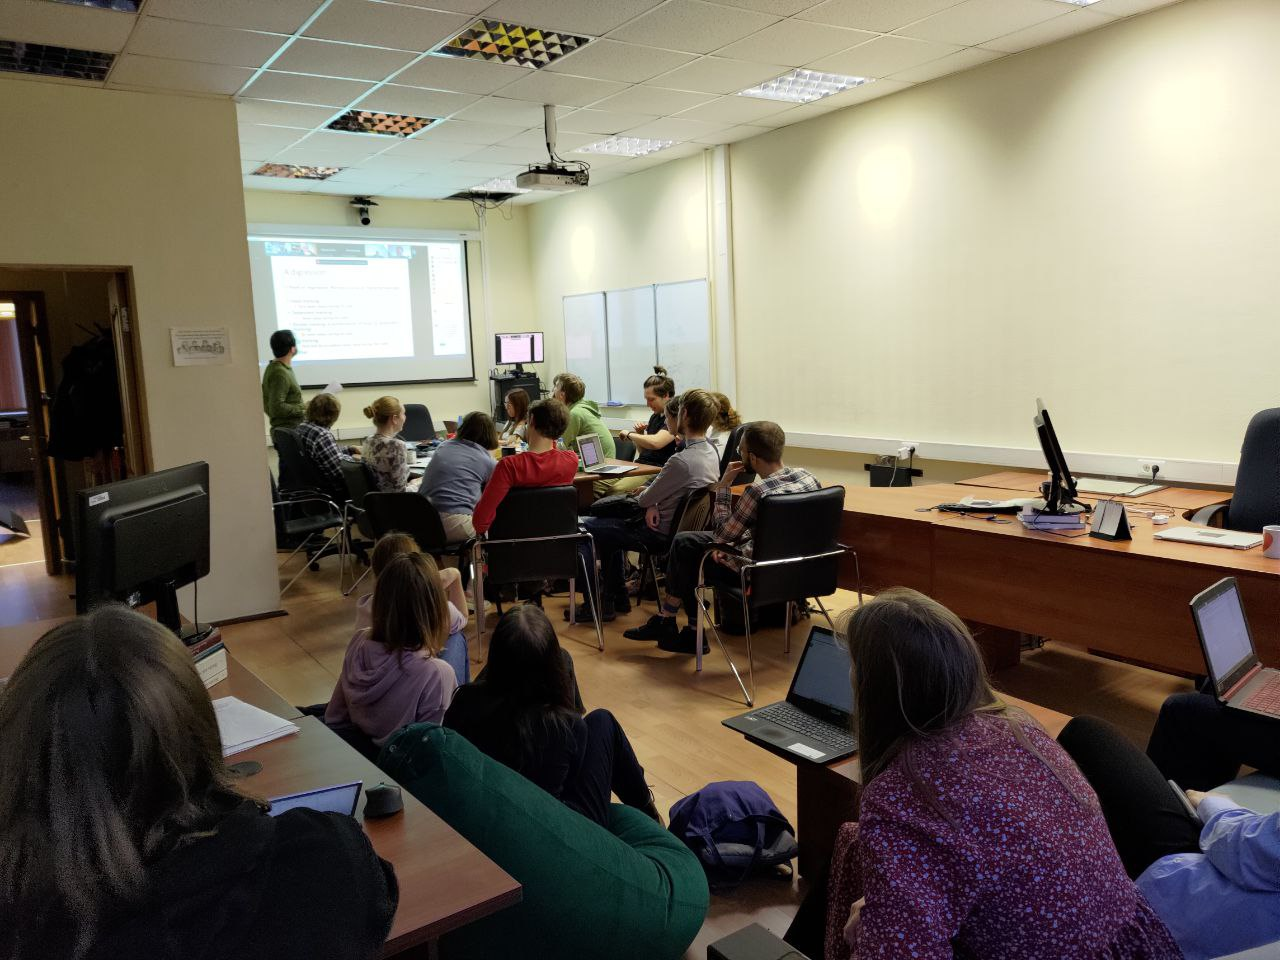
\includegraphics[width=0.9\linewidth]{images/06_seminar} \end{center}
\end{frame}

\begin{frame}{Школы, круглые столы, экспедиции}
\protect\hypertarget{ux448ux43aux43eux43bux44b-ux43aux440ux443ux433ux43bux44bux435-ux441ux442ux43eux43bux44b-ux44dux43aux441ux43fux435ux434ux438ux446ux438ux438}{}
\begin{itemize}
\tightlist
\item
  Онлайн школа по Нахско-дагестанским языкам (на английском языке,
  открытая, онлайн), 24 лекции
\item
  Международный воркшоп ``Emerging Topics in Typology'' (между 25
  октября и 22 ноября 2021, онлайн)
\item
  Воркшоп ``Spatial and social separation of speech communities and
  language change'' на 55-ом съезде европейского лингвистического
  общества (24--27 августа 2022, Бухарест)
\item
  Онлайн курс по азербайджансокму Мурада Сулейманова (École Pratique des
  Haute Études, 2020)
\item
  Два выезда российского общества полевых лингвистов (март и октябрь
  2022)
\item
  Около 20 экспедиций по исследованию малых языков и сбору данных в
  Дагестан, Адыгею, Карачаево-Черкесию, Кабардино-Балкарию, Чукотку и
  Сахалин \pause
\item
  Планируем в следующем году устроить школу по корпусным исследованиям
\end{itemize}
\end{frame}

\begin{frame}{Защиты диссертаций}
\protect\hypertarget{ux437ux430ux449ux438ux442ux44b-ux434ux438ux441ux441ux435ux440ux442ux430ux446ux438ux439}{}
\begin{itemize}
\tightlist
\item
  Из трех заявленых защит состоялась лишь одна:

  \begin{itemize}
  \tightlist
  \item
    А. Н. Закирова должна предзащититься 19 декабря 2022
  \item
    А. В. Яковлева защитилась 25 октября 2021
  \end{itemize}
\item
  В данный момент в лаборатории работают еще четыре аспиранта
\end{itemize}

\begin{center}
\includegraphics[width=0.8\linewidth]{images/07_yakovleva} \end{center}
\end{frame}

\begin{frame}{Привлеченные средства}
\protect\hypertarget{ux43fux440ux438ux432ux43bux435ux447ux435ux43dux43dux44bux435-ux441ux440ux435ux434ux441ux442ux432ux430}{}
\begin{itemize}
\tightlist
\item
  Запланировано 15 млн, получилось 17.5 млн
\item
  2018 -- 2020 Грант РФФИ (18-012-00852А) ``Морфосинтаксис андийского
  языка: опыт внутригенетической типологии``
\item
  2018 -- 2021 Грант РНФ (18-78-10128) ``Когда глагол не глагол:
  нефинитные конструкции в языках России``
\item
  2019 -- 2022 Грант РНФ (19-78-10139) ``Аргументная структура, залог и
  актантная деривация в языках Западной Сибири''
\item
  Подана заявка на новый грант РНФ совместно со Школой лингвистики
  ``Лингвистические маркеры социальных изменений''
\end{itemize}
\end{frame}

\begin{frame}{Публикации}
\protect\hypertarget{ux43fux443ux431ux43bux438ux43aux430ux446ux438ux438}{}
\begin{itemize}
\tightlist
\item
  32 публикации (планировалось 24)
\item
  Включая 15 WoS Q1-Q2 (планировали 8)
\end{itemize}
\end{frame}

\begin{frame}{Будущие планы}
\protect\hypertarget{ux431ux443ux434ux443ux449ux438ux435-ux43fux43bux430ux43dux44b}{}
\begin{itemize}
\tightlist
\item
  Продолжать и поддерживать существующие проекты

  \begin{itemize}
  \tightlist
  \item
    исследование вариативности на материале имеющихся устных корпусов
  \item
    типологические исследования
  \end{itemize}
\item
  Совместная работа с региональными университетами по созданию новых
  устных корпусов русского языка

  \begin{itemize}
  \tightlist
  \item
    уже идет работа с Южным Федеральным Университетом в рамках
    зеркальной лаборатории
  \item
    контакты с Иркутским государственным университетом, вышкинским
    кампусом в Санкт Петербурге (заявка на межкампусное взаимодействие)
  \end{itemize}
\item
  Переориентация имеющихся ресурсов на конкретные продукты для малых
  языков

  \begin{itemize}
  \tightlist
  \item
    распознавание речи
  \item
    материалы и словари малых языков
  \item
    морфологические парсеры, спеллчекеры, предективный набор
  \end{itemize}
\end{itemize}
\end{frame}

\begin{frame}{}
\protect\hypertarget{section}{}
\LARGE Спасибо за внимание!
\end{frame}

\end{document}
